\thispagestyle{plain}
\chapter{Σύνολα Δεδομένων και Προεπεξεργασία Εικόνων}
\label{chap:4}
\section{Σύνολα Δεδομένων}
\label{sec:4.1}

\subsection{Σύνολο Δεδομένων Kaggle}
\label{subsec:4.1.1}
Τα δεδομένα προέρχονται από ένα διαγωνισμό του Κaggle που διεξήχθη το 2015 και αφορούσε την διάγνωση της Διαβητικής Αμφιβληστροειδοπάθειας\cite{Kaggle}. Στο διαγωνισμό ζητήθηκε η διάγνωση της σοβαρότητας της ασθένειας για αυτό χρησιμοποιήθηκαν μοντέλα για ταξινόμηση πολλών κλάσεων. Το σύνολο δεδομένων είναι χωρισμένο σε πέντε κλάσεις ως εξής: 0 - No, 1 - Mild, 2 -Moderate, 3 - Severe, 4 - Proliferative.

Το σύνολο δεδομένων Kaggle αποτελείται από εικόνες υψηλής ανάλυσης διαφόρων διαστάσεων (433x289 μέχρι 5184x3456), οι οποίες έχουν τραβηχτεί σε διάφορες συνθήκες φωτισμού και με διάφορα μοντέλα και τύπους κάμερας. Για κάθε ασθενή είναι διαθέσιμες εικόνες του αμφιβληστροειδούς και των δύο ματιών. Η αντιστοίχιση των εικόνων στις διάφορες κλάσεις έγινε από έναν κλινικό ιατρό.

To σύνολο εκπαίδευσης αποτελείται από 35126 εικόνες RGB, ενώ το σύνολο ελέγχου από 53576 εικόνες RGB. H κάθε εικόνα των παραπάνω συνόλων ανήκει σε μία από τις πέντε προαναφερθείσες κλάσεις. Τα δύο σύνολα ενώθηκαν και στη συνέχεια χωρίστηκαν εκ νέου στα σύνολα: εκπαίδευσης,  επικύρωσης και ελέγχου. Παρακάτω θα γίνει μία συνοπτική περιγραφή του διαχωρισμού του συνόλου δεδομένων ενώ για περισσότερη παραστατικότητα παρατίθεται η εικόνα \ref{figure:data}.
\begin{figure}[!h]
    \centering
      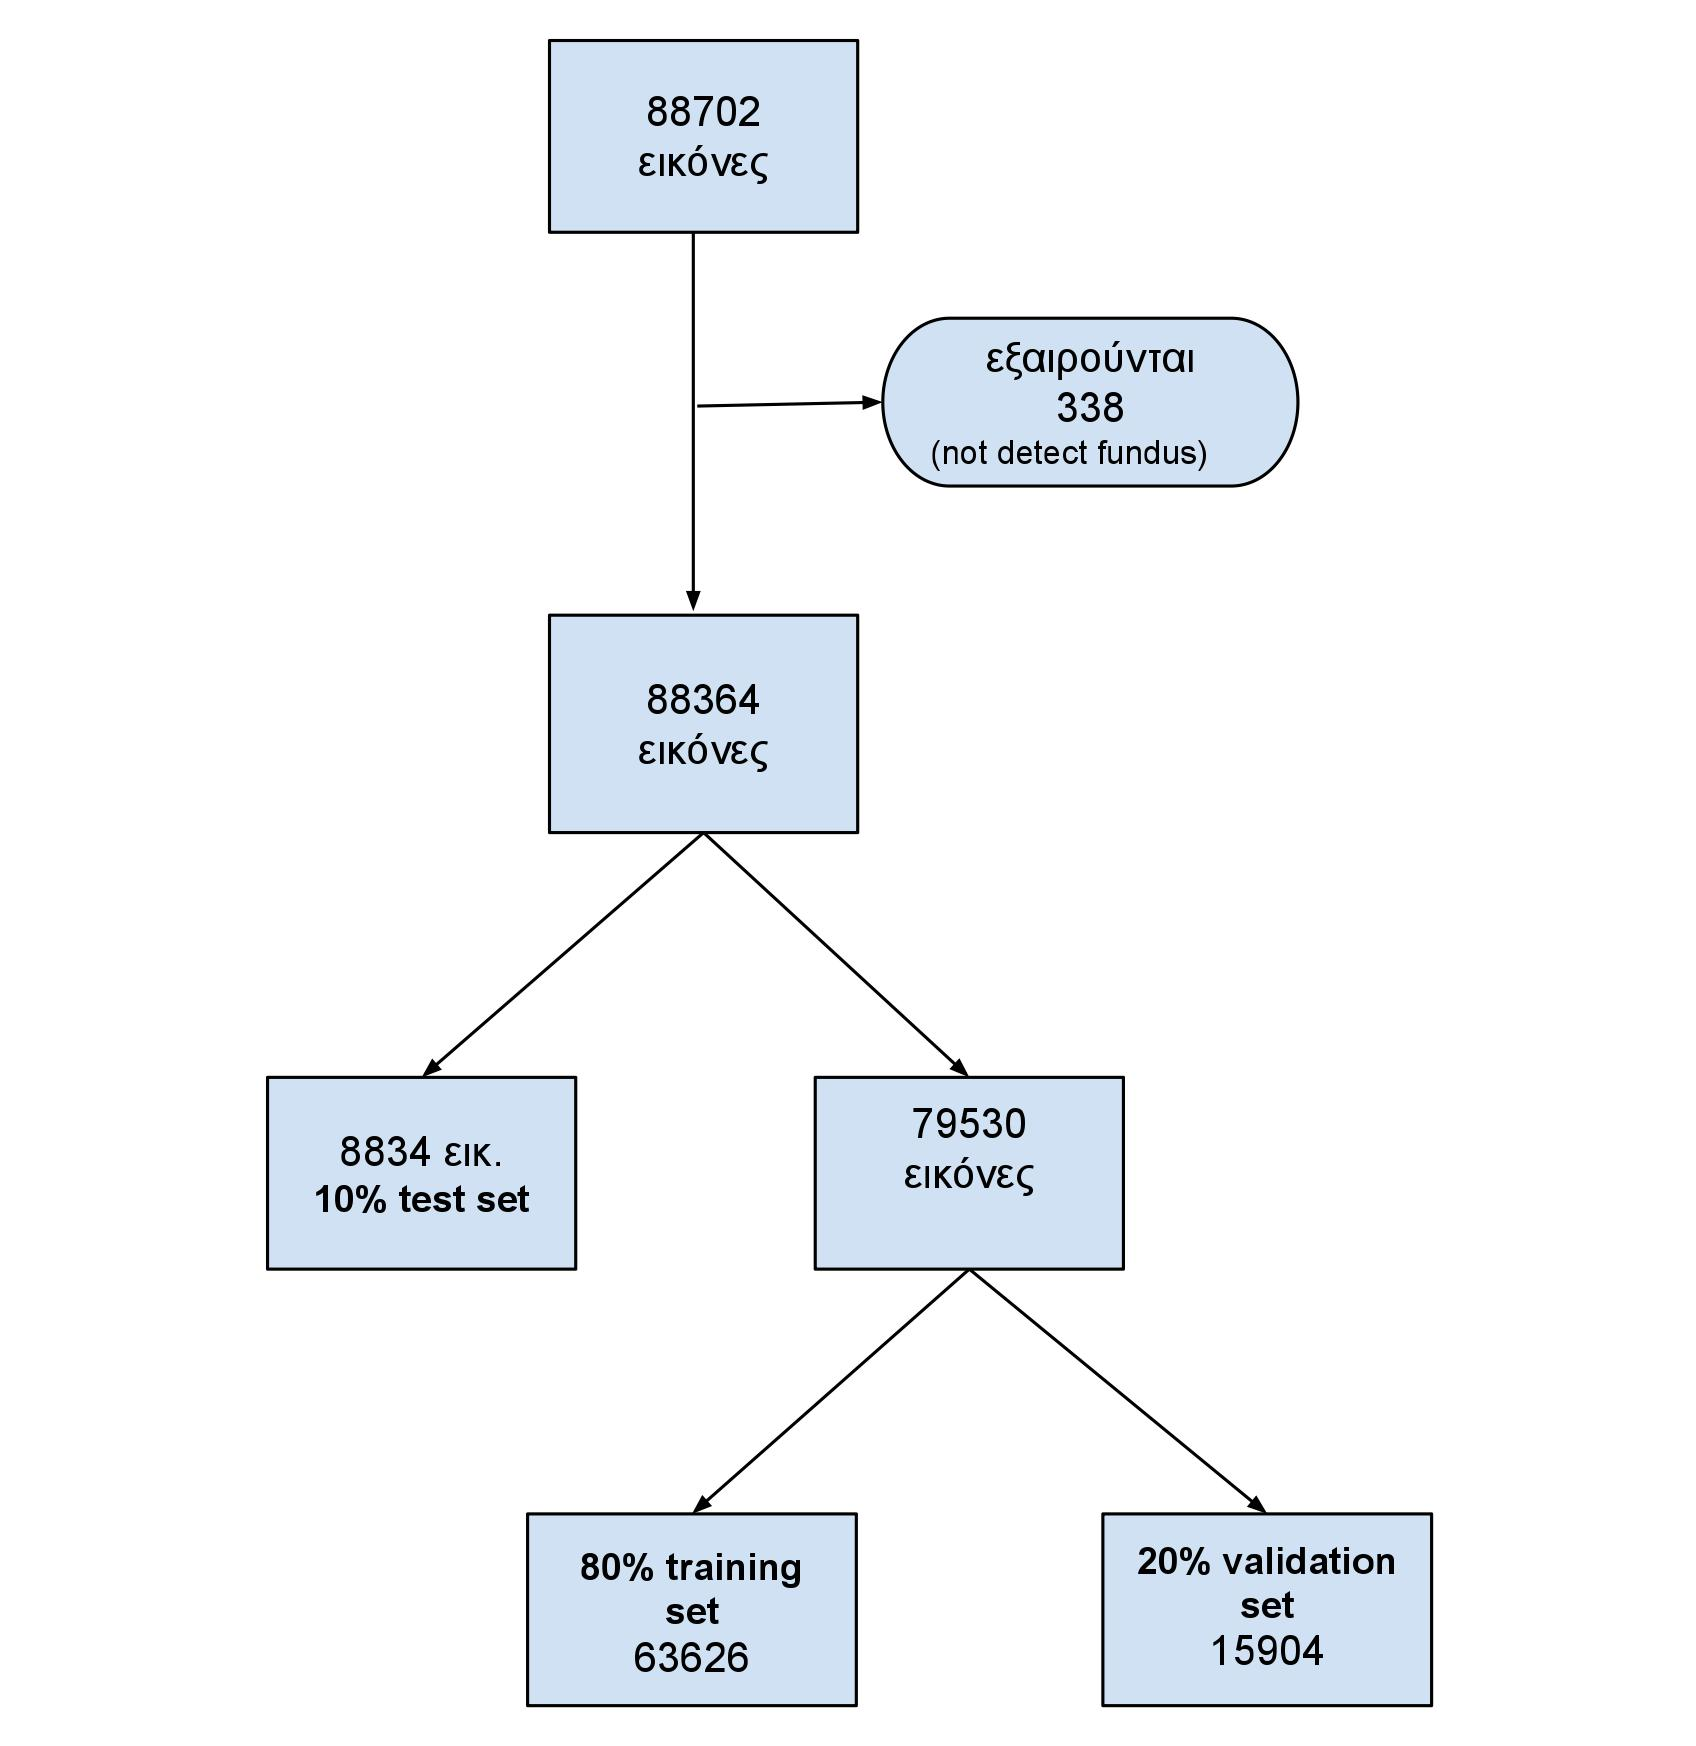
\includegraphics[width=0.9\linewidth]{data.jpg} \caption{ Διαχωρισμός του συνόλου δεδομένων στα σύνολα εκπαίδευσης, επικύρωσης και ελέγχου}
\label{figure:data}    
  \end{figure}

Αρχικά, το ενοποιημένο σύνολο αποτελείται από 88702 εικόνες και η κάθε εικόνα ανήκει σε μία από τις πέντε κλάσεις. Μετά την εφαρμογή του μετασχηματισμού Hough,  οι εικόνες στις οποίες δεν ανιχνεύεται ο αμφιβληστροειδής, εξαιρούνται. Οπότε καταλήγουμε με 88364 εικόνες. Στη συνέχεια, επιλέγουμε τυχαία $10\%$ των δεδομένων από κάθε κλάση για το σύνολο ελέγχου ενώ το υπόλοιπο $90\%$, διαχωρίζεται εκ νέου σε σύνολο εκπαίδευσης και σύνολο επικύρωσης με ποσοστά $80\%$ και $20\%$ από κάθε κλάση , αντίστοιχα.


Στο παραπάνω σύνολο δεδομένων υπάρχει θόρυβος ο οποίος οφείλεται στο γεγονός ότι η αντιστοίχιση των εικόνων στις κλάσεις έγινε μόνο από έναν κλινικό ιατρό και από την κακή ποιότητα ορισμένων εικόνων. Ορισμένες εικόνες έχουν τραβηχθεί σε συνθήκες χαμηλής ή υψηλης έκθεσης, κακής εστίασης ενώ σε ορισμένες περιπτώσεις υπάρχει αλλοίωση του περιεχομένου της εικόνας.

Μόλις το $75\%$ των εικόνων θεωρείται βαθμολογήσιμο.\cite{Rakhlin} Οι υπόλοιπες εικόνες παρουσιάζουν κακή ποιότητα. Στην εικόνα \ref{figure:badquality} παρατίθενται μερικά παραδείγματα εικόνων κακής ποιότητας.  
\begin{figure}[!h]
    \centering
      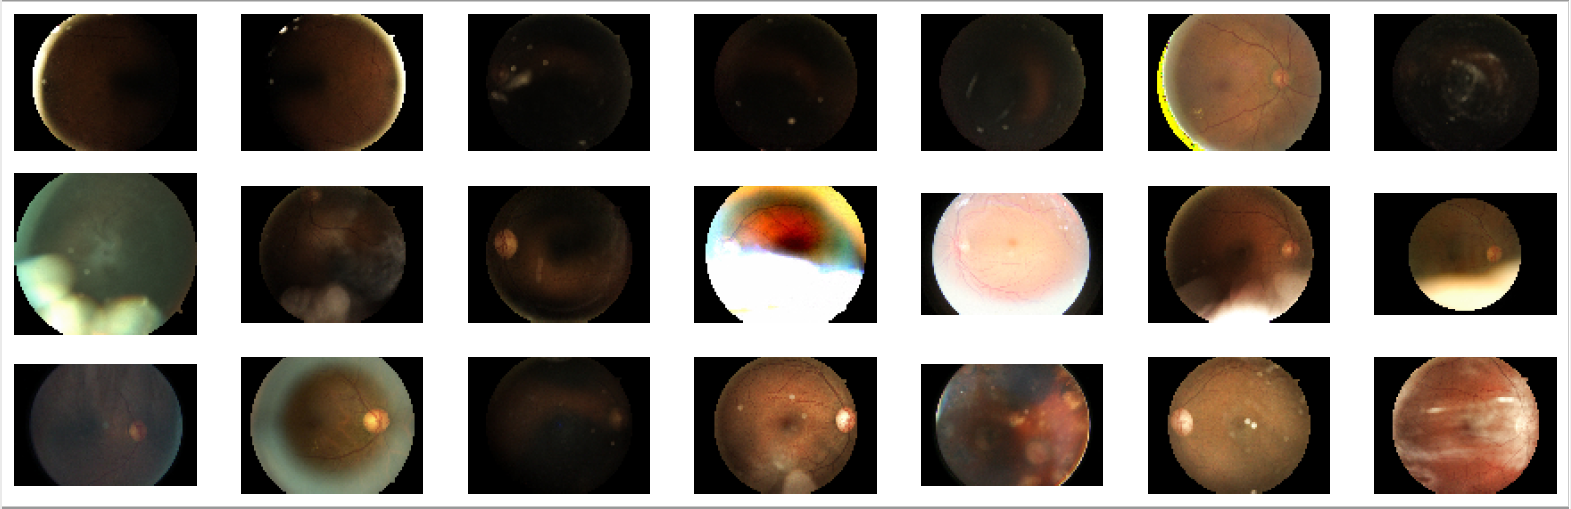
\includegraphics[width=1\linewidth]{badQuality.PNG} \caption{Εικόνες του συνόλου δεδομένων Kaggle που έχουν τραβηχτεί σε συνθήκες χαμηλής ή υψηλής έκθεσης, κακής εστίασης ενώ σε ορισμένες περιπτώσεις υπάρχει αλλοίωση του περιεχομένου της εικόνας}
 \label{figure:badquality}    
  \end{figure}


\subsection{Σύνολο Δεδομένων Messidor 2}
\label{subsec:4.1.2}
Το σύνολο δεδομένων Messidor 2 αποτελείται από 1748 εικόνες του αμφιβληστροειδούς. Η εικόνες έχουν ληφθεί με την κάμερα  Topcon TRC NW6 μη μυδριακής βάσης με οπτικό πεδίο 45 μοιρών και έχουν διαστάσεις 1440x960, 2240x1488 ή 2304x1536 εικονοστοιχεία. Αποτελεί μία επέκταση του συνόλου δεδομένων Messidor1\cite{Decencière}. Το Messidor2 χρησιμοποιήθηκε εξ ολοκλήρου ως ένα δεύτερο σύνολο ελέγχου.Στην εικόνα \ref{figure:mes}  παρουσιάζονται κάποια ενδεικτικά δείγματα του συνόλου δεδομένων Messidor 2.

\begin{figure}[!h]
    \centering
      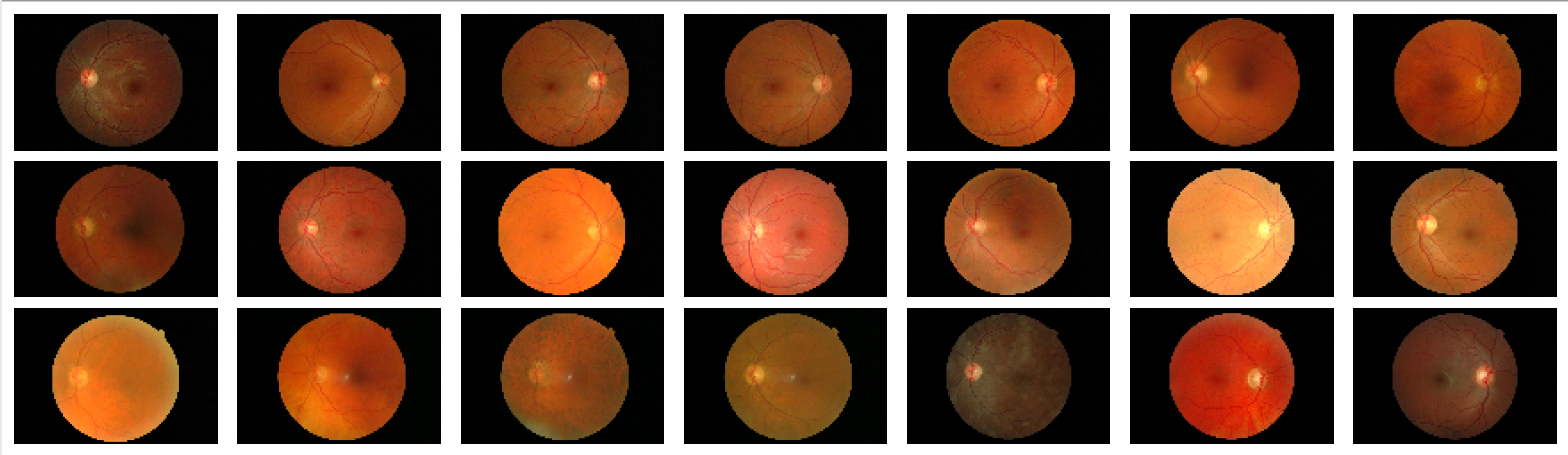
\includegraphics[width=1\linewidth]{mes3.PNG} \caption{Eνδεικτικά δείγματα του συνόλου δεδομένων Messidor 2}
\label{figure:mes}  
\end{figure}



\section{Προεπεξεργασία Εικόνων}
\label{sec:4.2}
\subsection{Διαδικασία Προεπεξεργασίας Εικόνων} 
\label{sec:4.2.1}
Για την επεξεργασία των εικόνων ακολουθείται η εξής διαδικασία. Αρχικά, μειώνονται οι διαστάσεις της εικόνας με σκοπό την ελάττωση του χρόνου επεξεργασίας, χωρίς ωστόσο να χαθεί η αναλογία. Στη συνέχεια εφαρμόζεται ο μετασχηματισμός Hough για την ανίχνευση του αμφιβληστροειδούς. Ο μετασχηματισμός Hough θα εξηγηθεί λεπτομερώς σε επόμενη παράγραφο. Επειδή, ο αλγόριθμος μπορεί να ανιχνεύσει πάνω από έναν κύκλους, η ακτίνα εύρεσης περιορίζεται στο διάστημα $[\frac{3mindim}{8},\frac{maxdim}{2}]$, όπου $mindim$ η μικρότερη διάσταση της εικόνας και $maxdim$ η μεγαλύτερη διάσταση της εικόνας. Το διάστημα αυτό υπολογίστηκε πειραματικά ώστε να καλύπτει όλες τις εικόνες. Επιπλέον, από τους κύκλους που ανιχνεύονται επιλέγεται ο πιο ισχυρός. Η επιλογή του πιο ισχυρού κύκλου σε συνδυασμό με τον περιορισμό του διαστήματος εύρεσης της ακτίνας, περιορίζει αρκετά το ενδεχόμενο λανθασμένης εύρεσης κύκλου. 

Το σύνολο δεδομένων Kaggle περιέχει δύο μορφές εικόνων, όπως μπορούμε να δούμε στην εικόνα \ref{figure:2morfes}. Η μία μορφή περιέχει ολόκληρο τον αμφιβληστροειδή ενώ η δεύτερη έχει κομμένο το πάνω και κάτω μέρος του αμφιβληστροειδούς.

\begin{figure}[!h]
\centering
\begin{subfigure}{.5\textwidth}
  \centering
  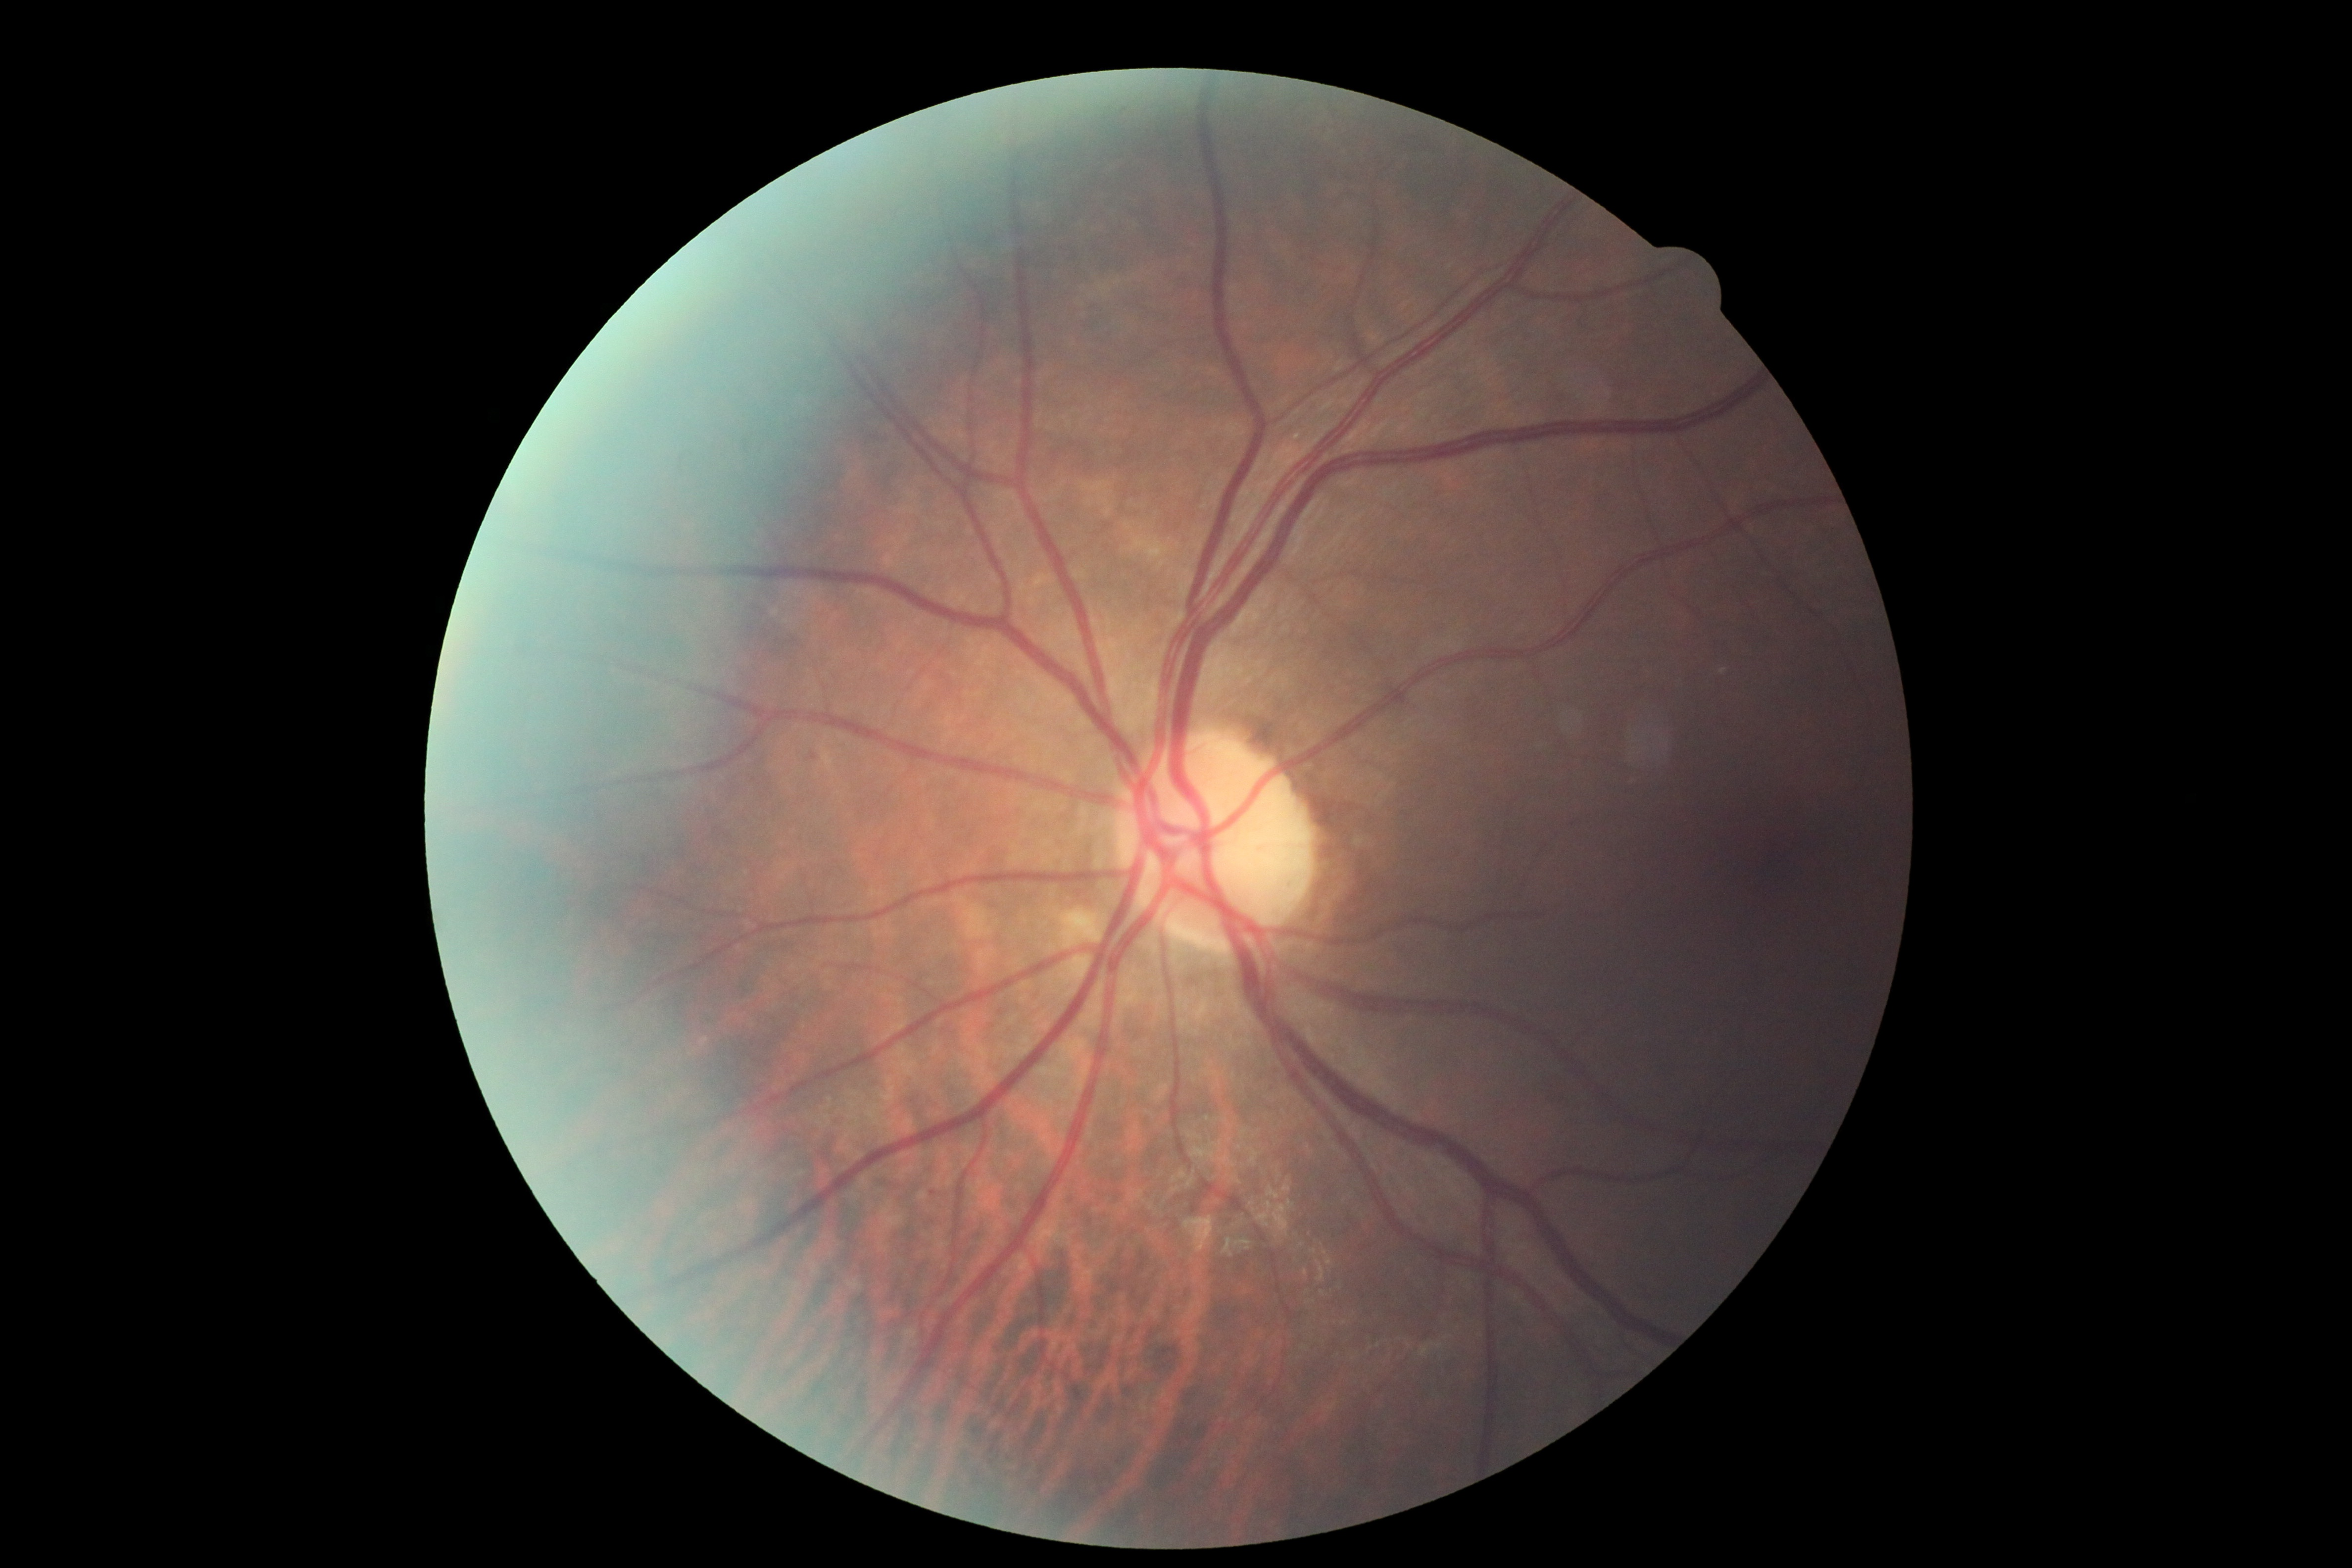
\includegraphics[width=0.8\linewidth]{1.jpeg}
  \caption{Ολόκληρος Αμφιβληστροειδής}
  \label{fig:2morfes1}
\end{subfigure}%
\begin{subfigure}{.5\textwidth}
  \centering
  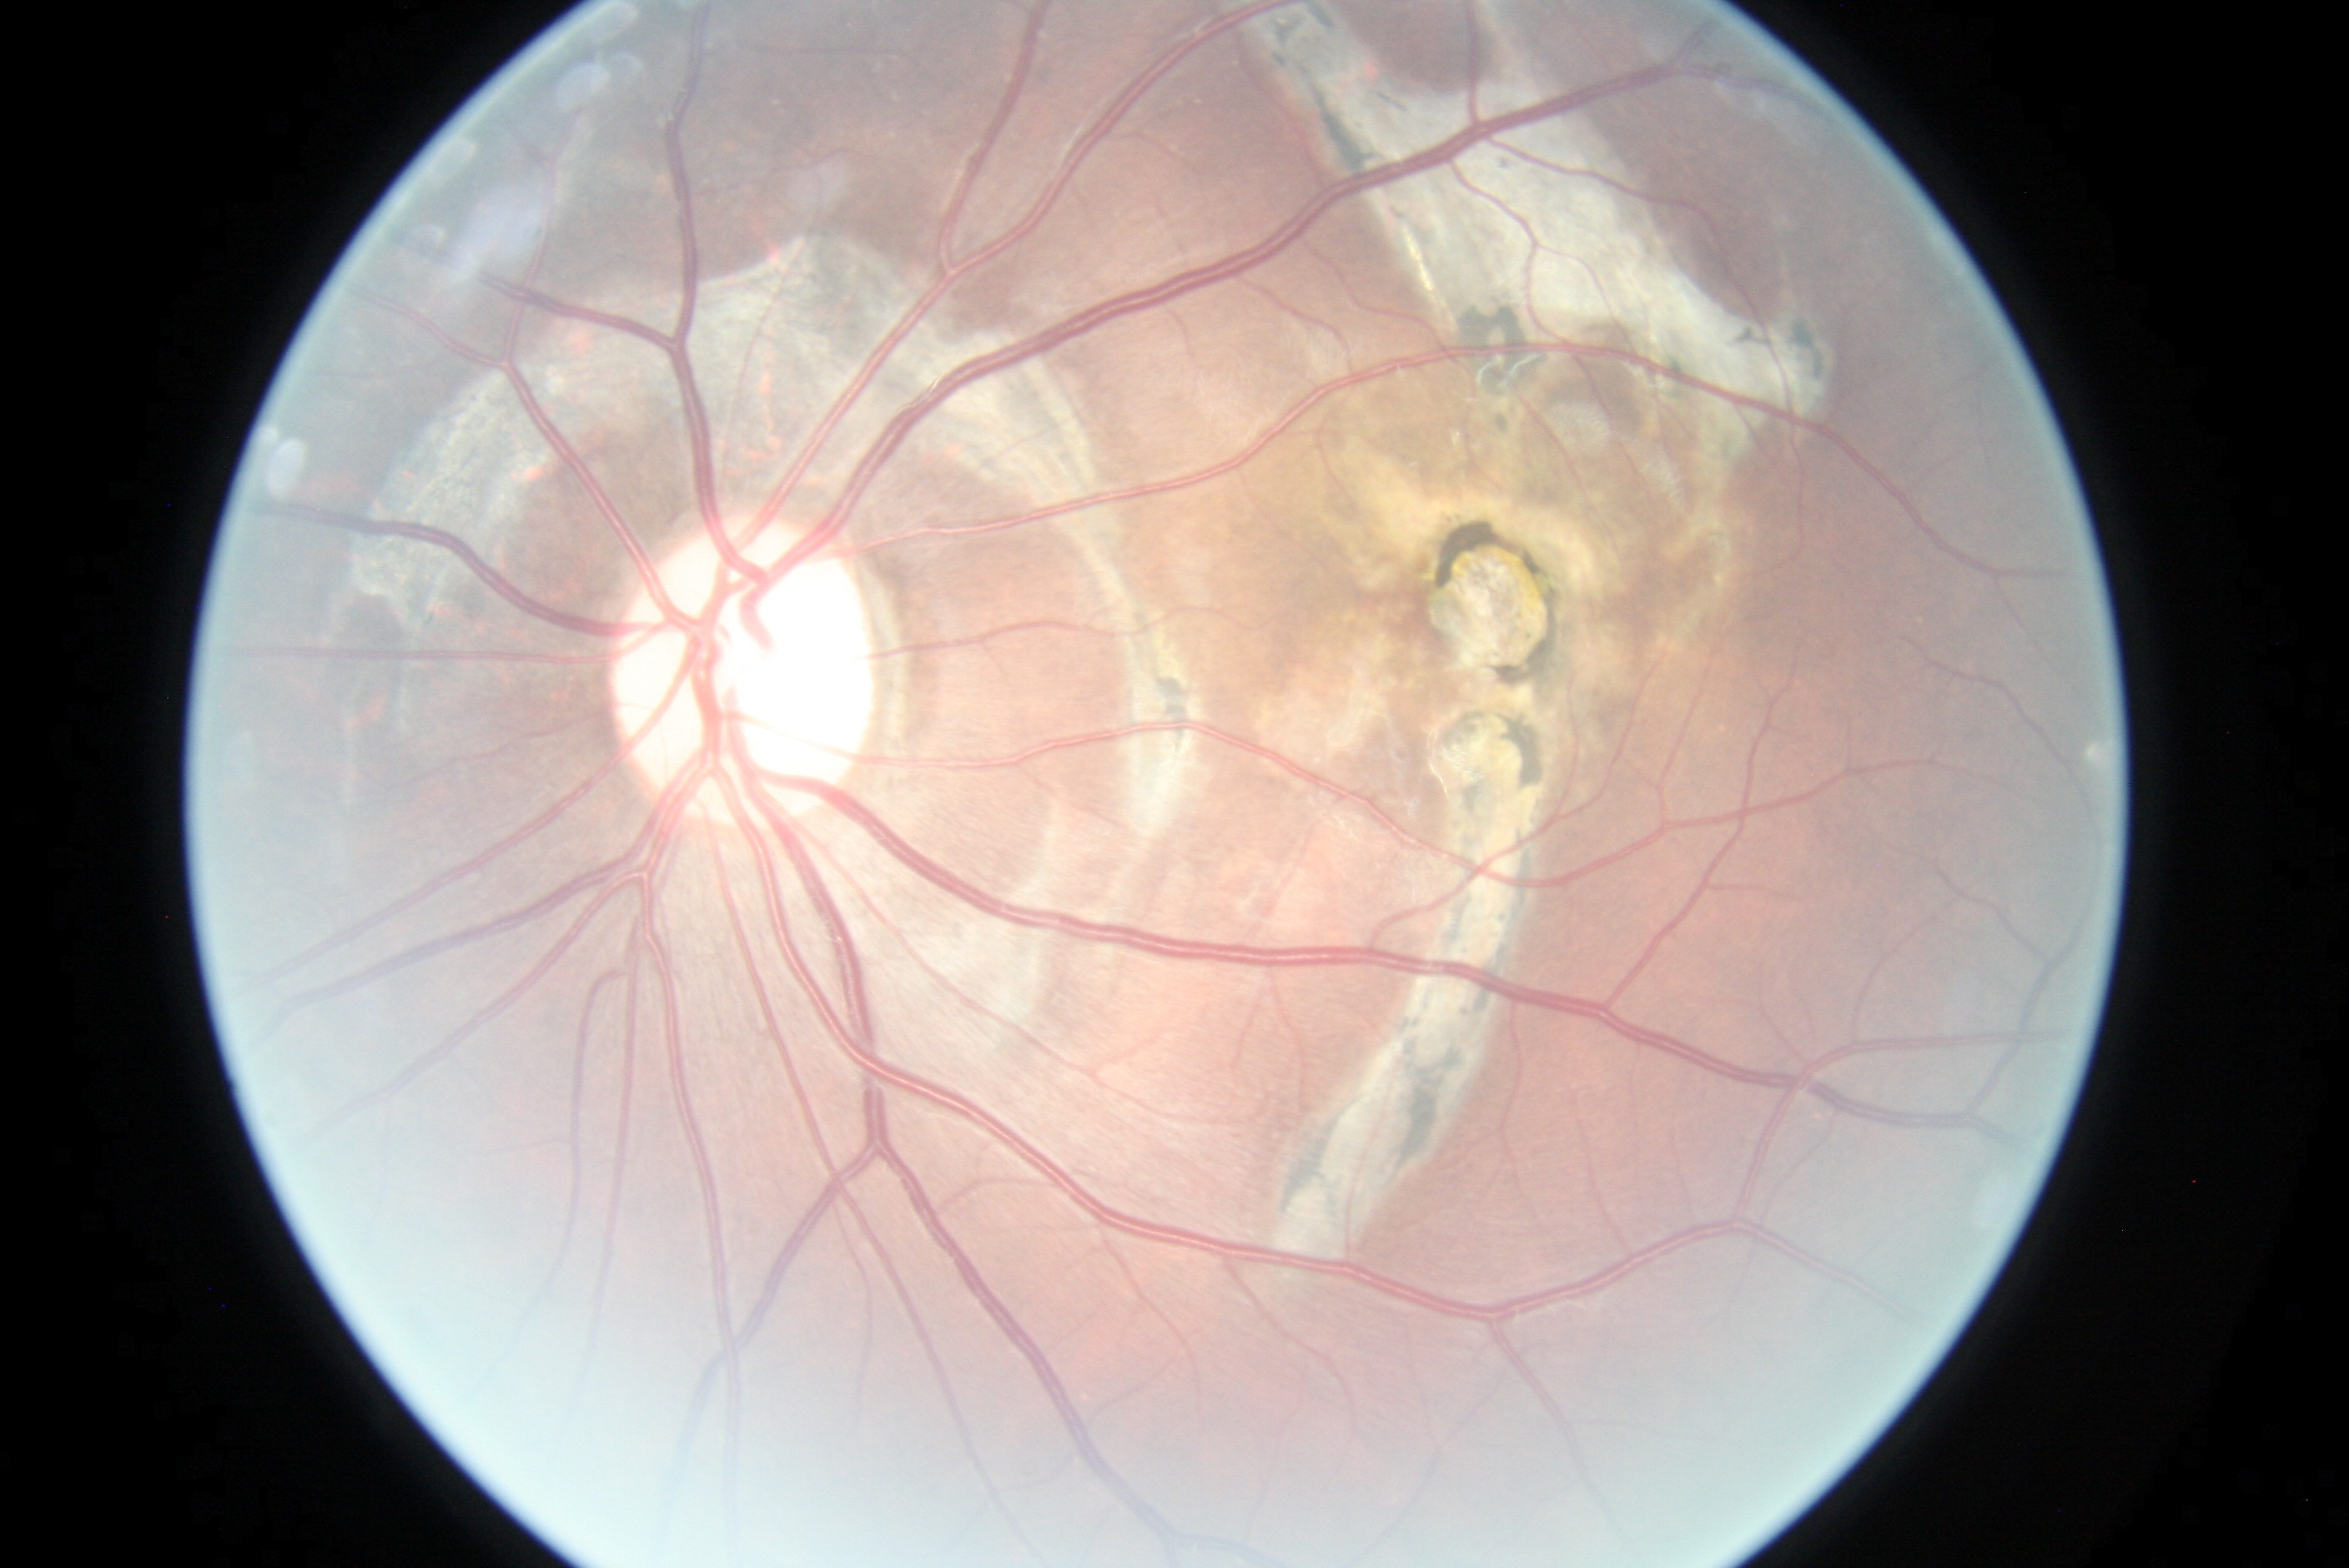
\includegraphics[width=0.8\linewidth]{2.jpeg}
  \caption{Κομμένος πάνω και κάτω Αμφιβληστροειδής}
  \label{fig:2morfes2}
\end{subfigure}
\caption{Δύο μορφές αμφιβληστροειδούς}
\label{figure:2morfes}
\end{figure}
  
Αφού βρεθεί το κέντρο και η ακτίνα του κύκλου με τον μετασχηματισμό Hough, κόβουμε την εικόνα με κέντρο το κέντρο του κύκλου, κρατώντας ένα παράθυρο με διαστάσεις [2ακτίνα x 2ακτίνα]. Στην περίπτωση του μη ολόκληρου αμφιβληστροειδούς ακολουθείται η ίδια διαδικασία με την διαφορά ότι στο πάνω και κάτω μέρος προστίθενται όσα μηδενικά απαιτούνται για να καταλήξουμε στην [2ακτίνα x 2ακτίνα] εικόνα. Τέλος, μειώνεται το μέγεθος της εικόνας, στο μέγεθος που θα δοθεί ως είσοδο στο νευρωνικό, δηλαδή $299x299$. Στην \ref{figure:kag3} και \ref{figure:mes3} παρουσιάζονται οι κομμένες εικόνες των συνόλων δεδομένων Kaggle και Messidor 2, αντίστοιχα.

\begin{figure}[!h]
    \centering
      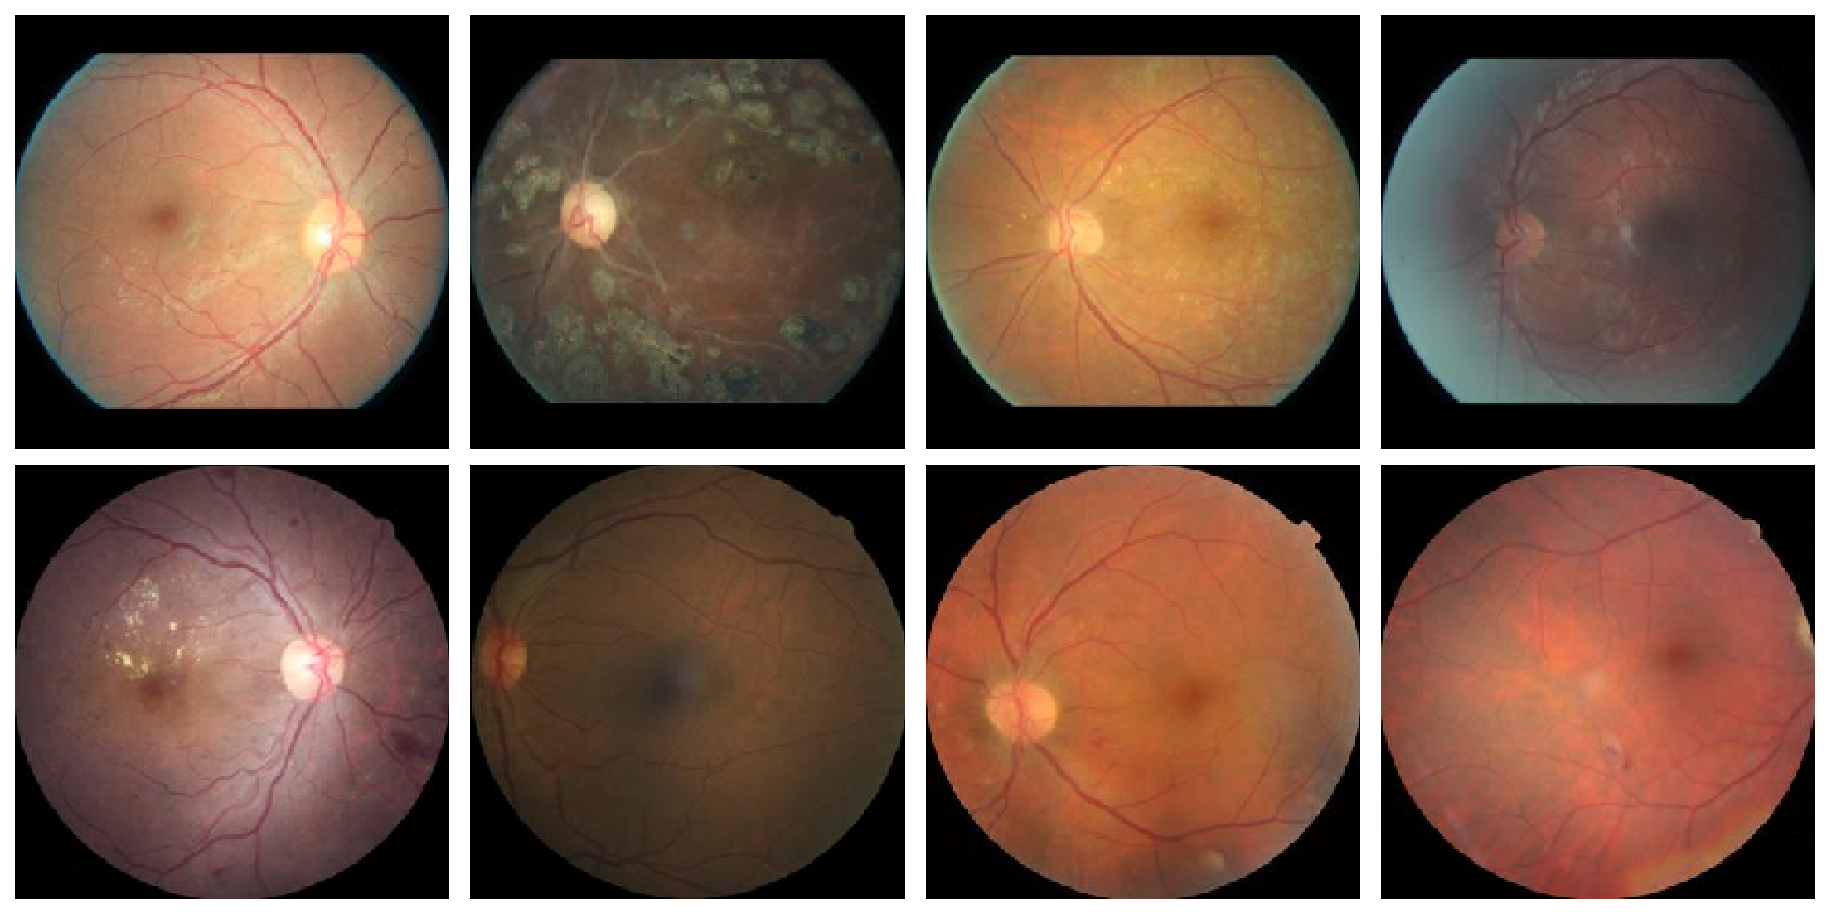
\includegraphics[width=1\linewidth]{kag3.pdf} \caption{Eνδεικτικά δείγματα κομμένων εικόνων του συνόλου δεδομένων Kaggle}
\label{figure:kag3}  
\end{figure}

\begin{figure}[!h]
    \centering
      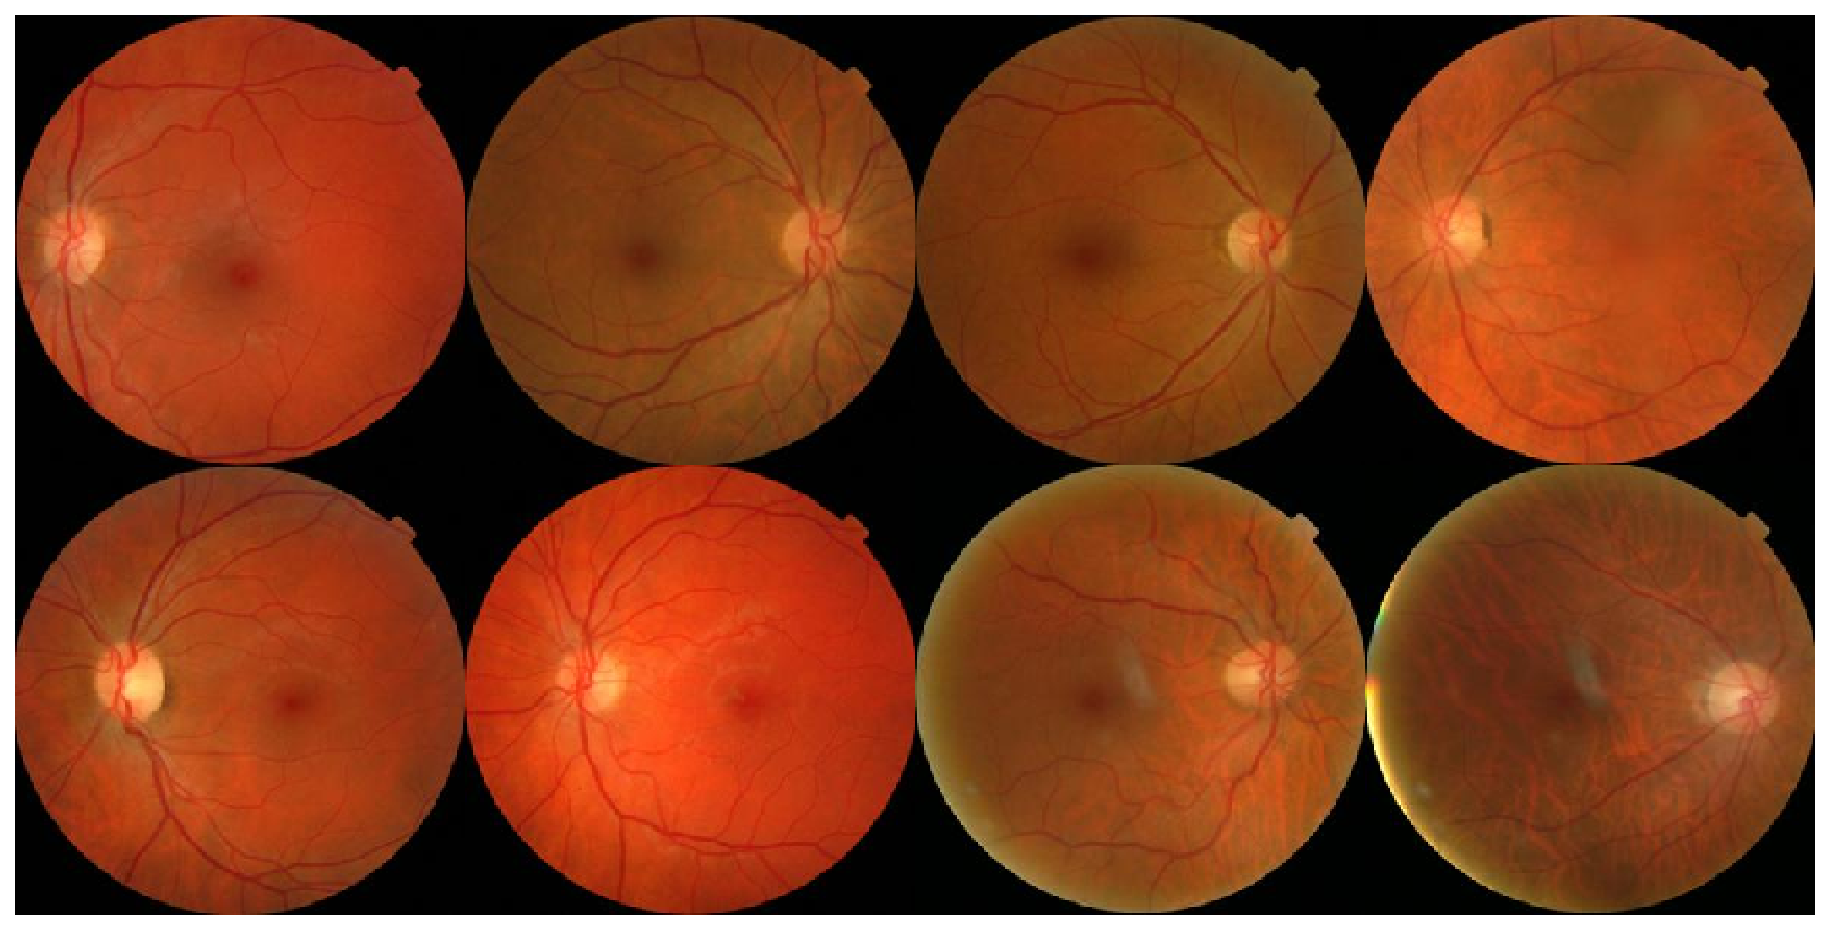
\includegraphics[width=1\linewidth]{mes.pdf} \caption{Eνδεικτικά δείγματα κομμένων εικόνων του συνόλου δεδομένων Messidor 2}
\label{figure:mes3}  
\end{figure}

\subsection{Μετασχηματισμός Hough} 
\label{sec:4.2.2}

Για την ανίχνευση του αμφιβληστροειδούς χρησιμοποιήθηκε ο μετασχηματισμός Hough\cite{Pedersen}. Ο μετασχηματισμός Hough μπορεί να περιγραφεί ως ένας μετασχηματισμός από το x,y επίπεδο, στο χώρο των παραμέτρων. Κάθε σχήμα απαιτεί διαφορετικό αριθμό παραμέτρων για να περιγραφεί, για αυτό ο μετασχηματισμός Hough χρησιμοποιείται συνήθως για απλά σχήματα των οποίων οι παράμετροι ανήκουν στο $R^2$ ή $R^3$. 
Ένα κύκλος μπορεί να περιγραφεί από την εξίσωση:
\begin{equation} \label{eq:circle}
r^2 =  (x - α)^2 + (y - β)^2
\end{equation}

Ο κύκλος έχει τρεις παραμέτρους, τις α, β και r που τα α, β αποτελούν το κέντρο του κύκλου στους άξονες x, y αντίστοιχα και r είναι η ακτίνα του κύκλου. Η παραμετρική εξίσωση του κύκλου είναι:

\begin{equation} \label{eq:par1}
x = α + r cos(\theta)
\end{equation}

\begin{equation} \label{eq:par2}
y = β + r cos(\theta)
\end{equation}

O χώρος των παραμέτρων ανήκει στο $R^3$. Κάθε σημείο του κύκλου στο xy επίπεδο, αντιστοιχίζεται στο χώρο των παραμέτρων σε κύκλους με κέντρο το συγκεκριμένο σημείο και ακτίνες σε ένα ορισμένο διάστημα. 


Εικονοστοιχεία με μεγάλη κλίση προδίδουν ύπαρξη ακμής οπότε είναι δυνατόν να ανήκουν σε κύκλο. Στην εικόνα\ref{figure:circle} παρουσιάζεται ο μετασχηματισμός Hough για τον μαύρο κύκλο. Κάθε διακεκομμένος κύκλος αποτελεί την αντιστοίχιση ενός σημείου του κύκλου από το x,y-επίπεδο, στο χώρο των παραμέτρων, για σταθερή ακτίνα. Να σημειωθεί ότι ενώ στην εικόνα επιλέγεται μία σταθερή ακτίνα για την καλύτερη γραφική αναπαράσταση, κάθε σημείο του κύκλου προβάλλεται σε k κύκλους με ίδιο κέντρο και ακτίνα που περιορίζεται σε ένα διάστημα.


\begin{figure}[!h]
    \centering
      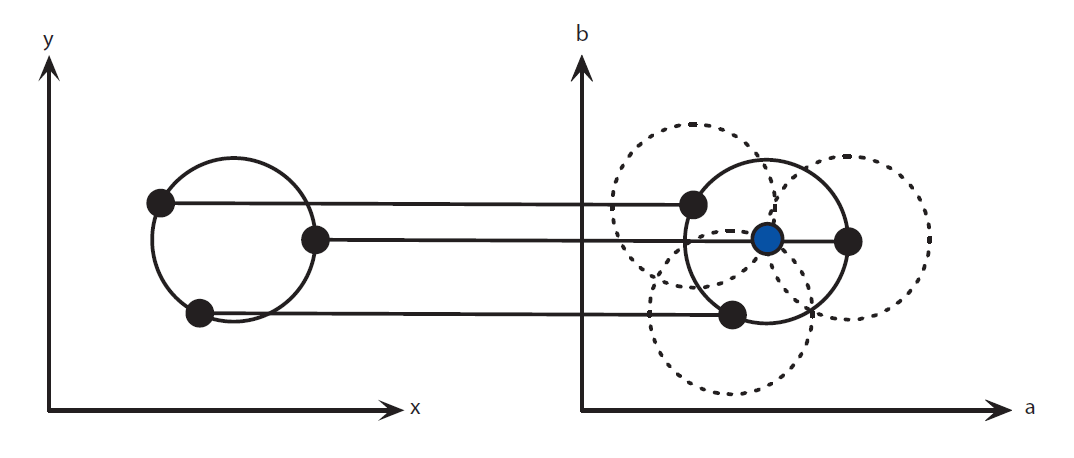
\includegraphics[width=0.5\linewidth]{hough2.PNG} \caption{Ο Μετασχηματισμός Hough από το x,y-επίπεδο(αριστερά), στο χώρο των παραμέτρων(δεξιά), για σταθερή ακτίνα}
\label{figure:circle}  
\end{figure}




Αν χωρίσουμε το χώρο σε ένα διακριτό πλέγμα, κάθε διακεκομμένος κύκλος ψηφίζει τα σημεία του. Όπως είναι φανερό το κέντρο του πραγματικού κύκλου θα βρίσκεται εκεί που θα υπάρχει μεγάλη συσσώρευση ψήφων καθώς οι διακεκομμένοι κύκλοι τέμνονται στο κέντρο του πραγματικού κύκλου.
Στην εικόνα \ref{figure:hough2} φαίνεται ο μετασχηματισμός Hough για μία εικόνα με 2 κύκλους. Ο μετασχηματισμός εφαρμόζεται για σταθερή ακτίνα r=20. Στο μετασχηματισμένο χώρο είναι φανερό ότι υπάρχει συσσώρευση ψήφων, στο κέντρο του πραγματικού κύκλου r=20. Καθώς το διάγραμμα είναι 2-d η συσσώρευση ψήφων αναπαριστάται με κόκκινο χρώμα. Επιπλέον, να σημειωθεί ότι το κέντρο του κύκλου με ακτίνα r = 25 δεν αναπαριστάται στο επίπεδο παραμέτρων, καθώς ο μετασχηματισμός Hough υπολογίστηκε για σταθερή ακτίνα r = 20.

\begin{figure}[!h]
\centering
\begin{subfigure}{.5\textwidth}
  \centering
  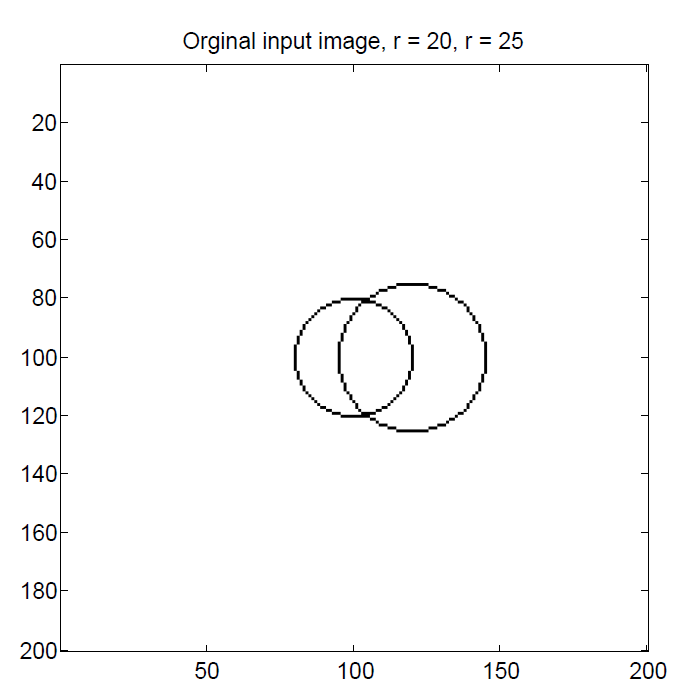
\includegraphics[scale=0.5]{h1.PNG}
  \caption{Εικόνα εισόδου}
  \label{fig:sub1bnew}
\end{subfigure}%
\begin{subfigure}{.4\textwidth}
  \centering
  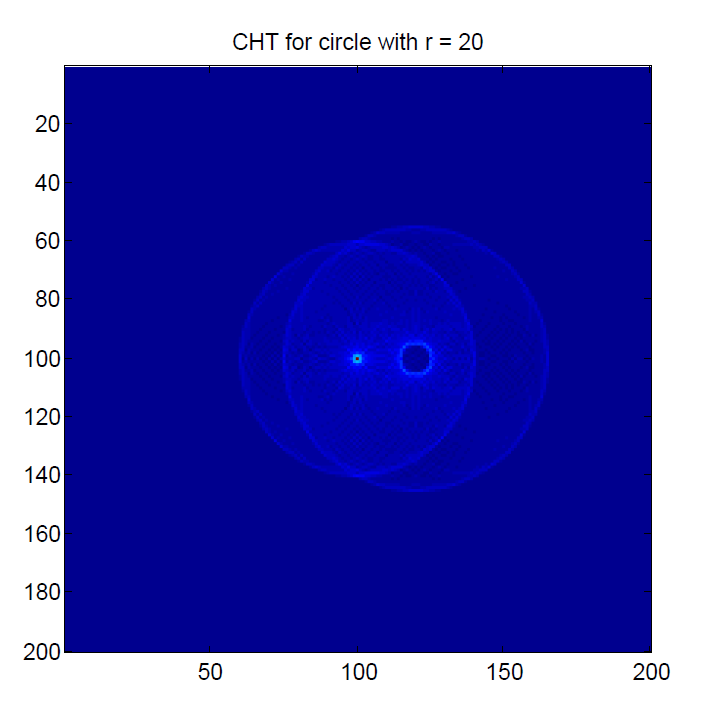
\includegraphics[scale=0.5]{h2.PNG}
  \caption{Μετασχηματισμός Hough για r = 20}
  \label{fig:sub2bnew}
\end{subfigure}
\caption{ Παράδειγμα συσσωρευτή του Μετασχηματισμού Hough για πραγματικά δεδομένα και σταθερή ακτίνα r = 20}
\label{figure:hough2}
\end{figure}



Για εύρεση κύκλου για μη σταθερή ακτίνα ακολουθείται η διαδικασία της ψηφοφορίας 
όπως περιγράφηκε για τη σταθερή ακτίνα με την προσθήκη ότι πια για κάθε κέντρο, υπάρχουν πολλοί κύκλοι λόγω της μη σταθερής ακτίνας. Οπότε πρέπει να επαναληφθεί ο αλγόριθμος της σταθερής ακτίνας για κάθε διαφορετική ακτίνα στο διάστημα που ορίστηκε. Αφού εφαρμοστεί, ο αλγόριθμος καταλήγει σε τριπλέτες $(α,β,r)$ για τους κύκλους που βρέθηκαν.


